\subsection{Formula dei trapezi composita}\label{subsection: formula dei trapezi composita}

Data la proprietà di additività dell'integrale:
\begin{equation*}
	I\left(f\right) = \displaystyle\sum_{k=1}^{M} \int_{I_{k}} f\left(x\right) \:\mathrm{d}x
\end{equation*}
Si vuole approssimare l'area sottesa da $f$ nell'intervallo $I_{k}$ considerando il trapezio costruito sui punti $x_{k-1}$ e $x_{k}$ e sulle corrispondenti ordinate.

\highspace
La formula dei \definition{trapezi composita} è:
\begin{equation}
	I_{tr}\left(f\right) = \dfrac{H}{2} \displaystyle\sum_{k=1}^{M} \left(f\left(x_{k-1}\right) + f\left(x_{k}\right)\right)
\end{equation}
Per comodità di implementazione, è possibile riscriverla anche come:
\begin{equation*}
	I_{tr}\left(f\right) = \dfrac{H}{2} \left(f\left(a\right) + f\left(b\right)\right) + H \sum_{k=1}^{M-1} f\left(x_{k}\right)
\end{equation*}
\begin{figure}[!htp]
	\centering
	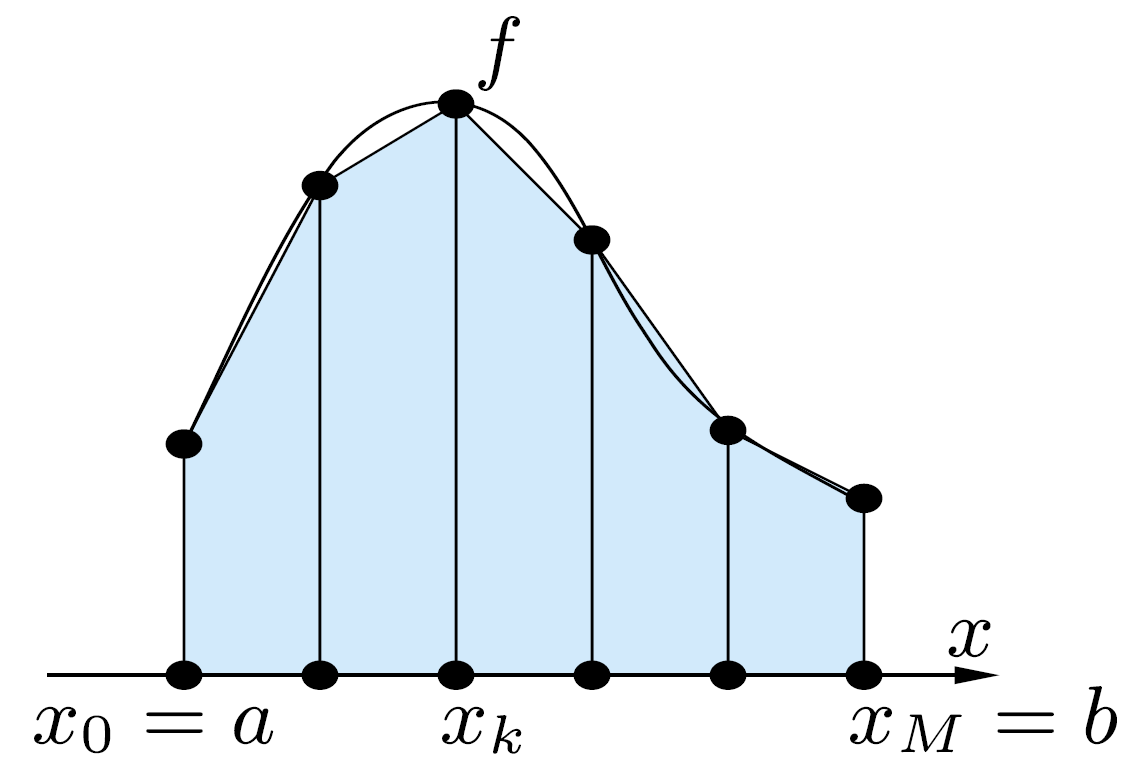
\includegraphics[width=.4\textwidth]{img/formule-di-quadratura-3.png}
\end{figure}

\noindent
Da notare che la formula dei trapezi composita equivale all'\textbf{integrale esatto dell'interpolatore Lagrangiano composito di grado 1}:
\begin{equation}
	I_{tr}\left(f\right) = \displaystyle \int_{a}^{b} \left(\displaystyle\prod_{1}^{H} f\left(x\right)\right) \:\mathrm{d}x
\end{equation}
Su ogni intervallo $I_{k}$ si può considerare l'errore di interpolazione Lagrangiana. 

\highspace
La \definition{stima dell'errore per la formula dei trapezi composita} è:
\begin{equation}
	\left|I\left(f\right) - I_{tr}\left(f\right)\right| \le \dfrac{1}{12} \underset{x}{\max} \left|f''\left(x\right)\right| \left(b-a\right) H^{2}
\end{equation}
Si possono fare due \textbf{osservazioni} riguardo alla stima dell'errore:
\begin{enumerate}
	\item La \textbf{formula dei trapezi composita} è di \textbf{ordine 2}.
	
	\item La \textbf{formula dei trapezi composita} ha \textbf{grado di esattezza pari a 1}.
\end{enumerate}
Da notare che sia grado che ordine sono uguali al punto medio composita. Per cui, \example{è meglio scegliere questo metodo o il punto medio?} La scelta risiede principalmente sull'\textbf{avere a disposizione le coordinate dei punti medi o dei punti estremi degli intervalli}.